\documentclass{beamer}

\newenvironment{tightcenter}{%
  \setlength\topsep{0pt}
  \setlength\parskip{0pt}
  \begin{center}
}{%
  \end{center}
}

\newenvironment{Snippet}{\Verbatim[samepage=true,fontsize=\footnotesize]}{\endVerbatim}

\mode<presentation>
{
  \usetheme{Copenhagen}
  %%\usecolortheme[RGB={173,222,25}]{structure}
  \usecolortheme[RGB={255,0,0}]{structure}
  \setbeamertemplate{items}[circle]
  \setbeamercovered{transparent}
}

\usepackage[polish]{babel}
\usepackage{hyperref}
\usepackage{qtree}
\usepackage{mathtools}
\usepackage{dirtytalk}
\usepackage{epigraph}
\usepackage[utf8]{inputenc}
\usepackage{times}
\usepackage[T1]{fontenc}
\usepackage{tikz}
\usepackage{csquotes}
\usepackage{amsmath}
\usepackage{fancyvrb}
\usepackage{ulem}
\usepackage{adjustbox}
\usepackage{array}
\usepackage{makecell}

\newcommand{\soutthick}[1]{%
  \renewcommand{\ULthickness}{2mm}%
  \sout{#1}%
  \renewcommand{\ULthickness}{.4pt}% Resetting to ulem default
}

\makeatletter
\newcommand{\crossout}[1]{%
  \begingroup
  \settowidth{\dimen@}{#1}%
  \setlength{\unitlength}{0.05\dimen@}%
  \settoheight{\dimen@}{#1}%
  \count@=\dimen@
  \divide\count@ by \unitlength
  \begin{picture}(0,0)
    \linethickness{2mm}
    \put(0,0){\line(20,\count@){20}}
    \put(0,\count@){\line(20,-\count@){20}}
  \end{picture}%
  #1%
  \endgroup
}
\makeatother

\renewcommand\theadalign{bc}
\renewcommand\theadfont{\bfseries}
\renewcommand\theadgape{\Gape[4pt]}
\renewcommand\cellgape{\Gape[4pt]}


\setbeamercovered{invisible}

\title{\textbf{Dobre praktyki, których nie ma na embedded}}

\author{Panicz Maciej Godek}

\institute{
  \tiny{\href{mailto:godek.maciek@gmail.com}{\textbf{godek.maciek@gmail.com}}}
}

\date{\textbf{Gdańsk Embedded Meetup\#5}, 04.02.2020}


\begin{document}

\begin{frame}
  \titlepage
\end{frame}


\begin{frame}[plain]
  \begin{center}
    \Huge
    \pause
    Bój się Boga \\
    \pause
    którego nie ma \\
    \pause
    w Twoim sercu
  \end{center}  
\end{frame}

\begin{frame}[plain]
  \begin{center}
    \Huge
    Bój się Boga \\
    \crossout{\soutthick{którego nie ma}} \\
    w Twoim sercu
  \end{center}
\end{frame}

\begin{frame}[plain]
  \begin{center}
    \Huge
    Dobre praktyki \\
    których nie ma \\
    na embedded
  \end{center}
\end{frame}

\begin{frame}[plain]
  \begin{center}
    \Huge
    Dobre praktyki \\
    \crossout{\soutthick{których nie ma}} \\
    na embedded
  \end{center}
\end{frame}


{ % all template changes are local to this group.
  \setbeamertemplate{navigation symbols}{}
  \begin{frame}[plain]
    \begin{tikzpicture}[remember picture,overlay]
      \node[at=(current page.center)] {
        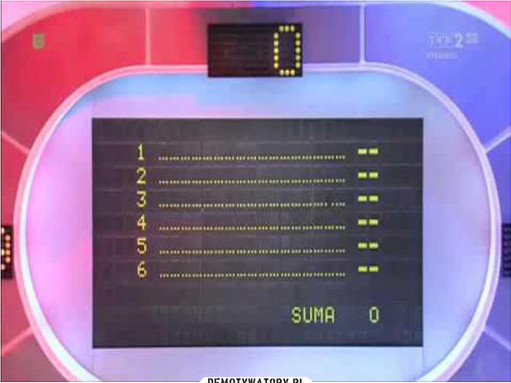
\includegraphics[width=\paperwidth,height=\paperheight]{familiada1.jpg}
      };
    \end{tikzpicture}
  \end{frame}
}

{ % all template changes are local to this group.
  \setbeamertemplate{navigation symbols}{}
  \begin{frame}[plain]
    \begin{tikzpicture}[remember picture,overlay]
      \node[at=(current page.center)] {
        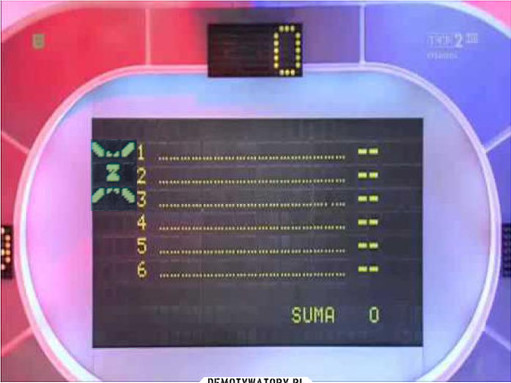
\includegraphics[width=\paperwidth,height=\paperheight]{familiada2.jpg}
      };
    \end{tikzpicture}
  \end{frame}
}

{ % all template changes are local to this group.
  \setbeamertemplate{navigation symbols}{}
  \begin{frame}[plain]
    \begin{tikzpicture}[remember picture,overlay]
      \node[at=(current page.center)] {
        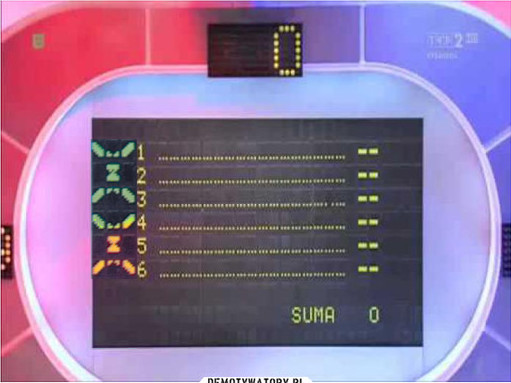
\includegraphics[width=\paperwidth,height=\paperheight]{familiada3.jpg}
      };
    \end{tikzpicture}
  \end{frame}
}

{ % all template changes are local to this group.
  \setbeamertemplate{navigation symbols}{}
  \begin{frame}[plain]
    \begin{tikzpicture}[remember picture,overlay]
      \node[at=(current page.center)] {
        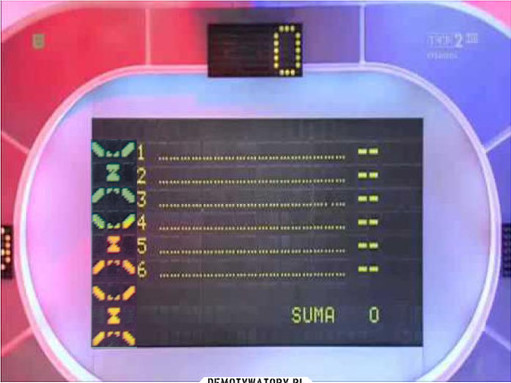
\includegraphics[width=\paperwidth,height=\paperheight]{familiada4.jpg}
      };
    \end{tikzpicture}
  \end{frame}
}

{ % all template changes are local to this group.
  \setbeamertemplate{navigation symbols}{}
  \begin{frame}[plain]
    \begin{tikzpicture}[remember picture,overlay]
      \node[at=(current page.center)] {
        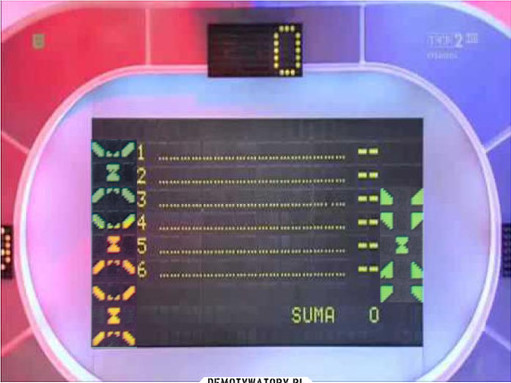
\includegraphics[width=\paperwidth,height=\paperheight]{familiada5.jpg}
      };
    \end{tikzpicture}
  \end{frame}
}

{ % all template changes are local to this group.
  \setbeamertemplate{navigation symbols}{}
  \begin{frame}[plain]
    \begin{tikzpicture}[remember picture,overlay]
      \node[at=(current page.center)] {
        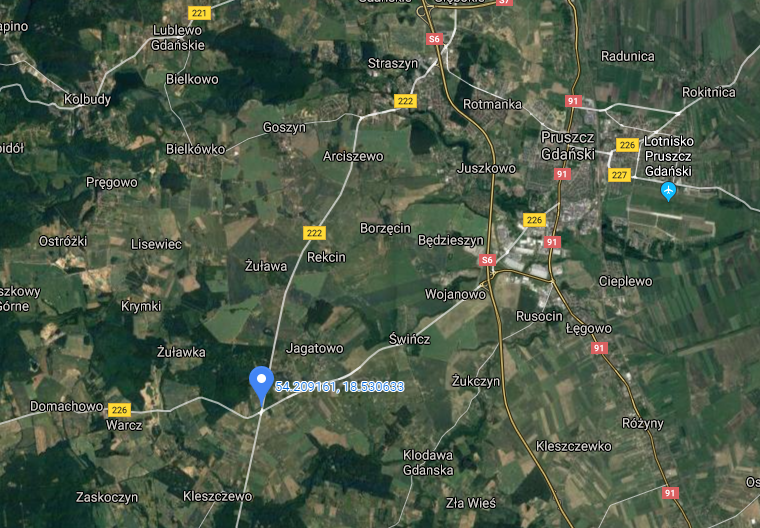
\includegraphics[width=\paperwidth,height=\paperheight]{jagatowo.png}
      };
    \end{tikzpicture}
  \end{frame}
}

{ % all template changes are local to this group.
  \setbeamertemplate{navigation symbols}{}
  \begin{frame}[plain]
    \begin{tikzpicture}[remember picture,overlay]
      \node[at=(current page.center)] {
        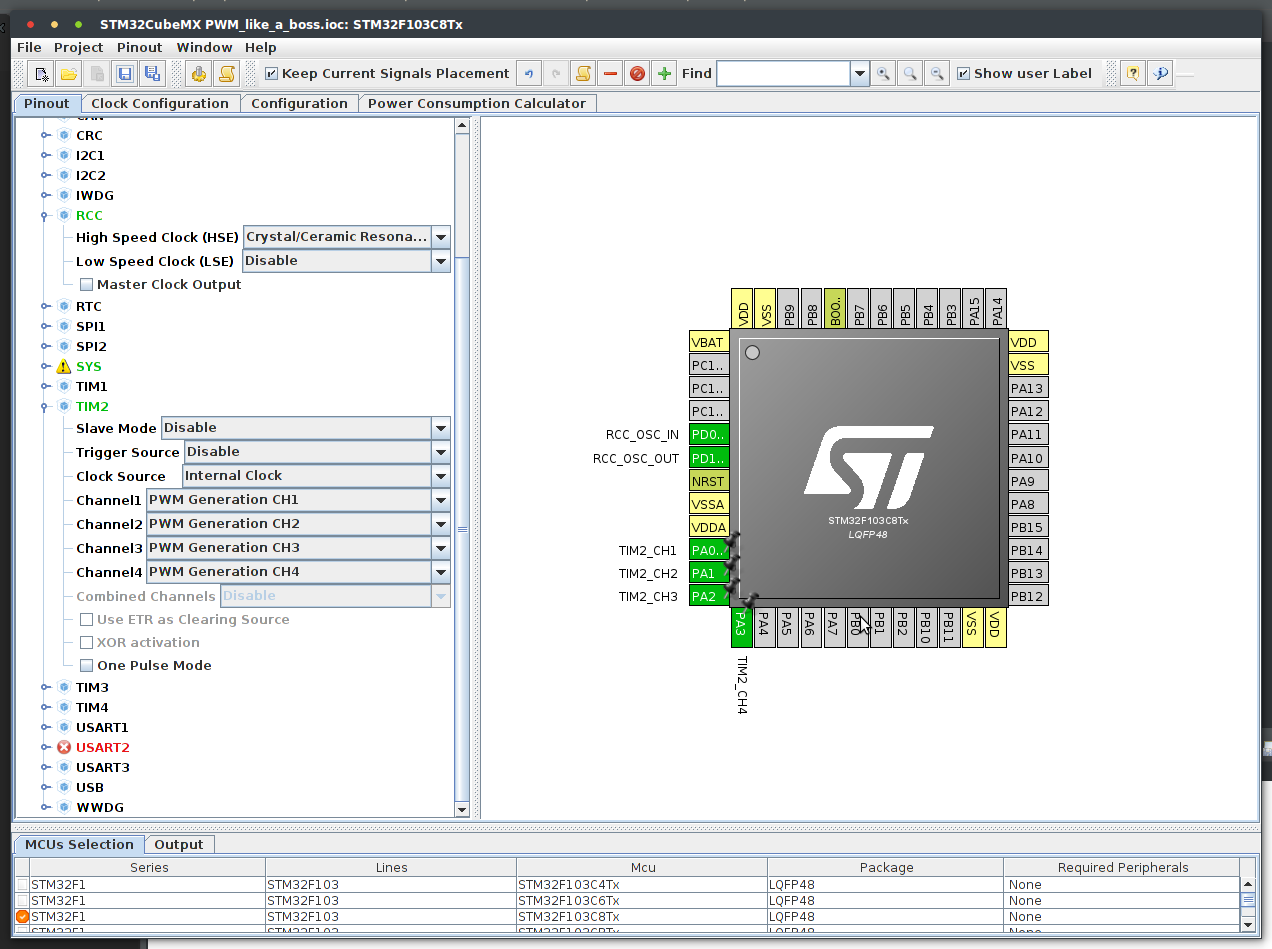
\includegraphics[width=\paperwidth,height=\paperheight]{cube.png}
      };
    \end{tikzpicture}
  \end{frame}
}

\begin{frame}[fragile]{Przykład złego interfejsu}
  \begin{Snippet}
HAL_StatusTypeDef HAL_RTC_GetTime(RTC_HandleTypeDef *hrtc,
                                  RTC_TimeTypeDef *sTime,
                                  uint32_t Format)
  \end{Snippet}
  \pause
  \begin{Snippet}
typedef struct {
    uint8_t Hours;
    uint8_t Minutes;
    uint8_t Seconds;
    uint8_t TimeFormat;
    uint32_t SubSeconds;
    uint32_t SecondFraction;
    uint32_t DayLightSaving;
    uint32_t StoreOperation;
} RTC_TimeTypeDef;
  \end{Snippet}
  \pause
  \begin{Snippet}
/* @param  Format: Specifies the format of the 
 *         entered parameters. This parameter can
 *         be one of the following values:
 *            @arg RTC_FORMAT_BIN: Binary data format
 *            @arg RTC_FORMAT_BCD: BCD data format */
  \end{Snippet}
\end{frame}

\begin{frame}[fragile]{Przykład złego interfejsu}
  \begin{Snippet}
/* @note You must call HAL_RTC_GetDate()
 *        after HAL_RTC_GetTime() to unlock
 *        the values in the higher-order
 *        calendar shadow registers to ensure
 *        consistency between the time
 *        and date values.
 *        Reading RTC current time locks
 *        the values in calendar shadow registers
 *        until current date is read. */
  \end{Snippet}
\end{frame}

\begin{frame}[fragile]{Inny przykład złego interfejsu}
  \begin{Snippet}
/**
 * @brief  Load the color lookup table.
 * @param  hltdc    pointer to a LTDC_HandleTypeDef
 *                  structure that contains the
 *                  configuration information for the LTDC.
 * @param  pCLUT    pointer to the color lookup table address.
 * @param  CLUTSize the color lookup table size.
 * @param  LayerIdx LTDC Layer index.
 *                  This parameter can be one
 *                  of the following values:
 *                  LTDC_LAYER_1 (0) or LTDC_LAYER_2 (1)
 * @retval HAL status
 */
 HAL_StatusTypeDef
 HAL_LTDC_ConfigCLUT(LTDC_HandleTypeDef *hltdc,
                     uint32_t *pCLUT,
                     uint32_t CLUTSize,
                     uint32_t LayerIdx)
  \end{Snippet}
\end{frame}

{ % all template changes are local to this group.
  \setbeamertemplate{navigation symbols}{}
  \begin{frame}[plain]
    \begin{tikzpicture}[remember picture,overlay]
      \node[at=(current page.center)] {
        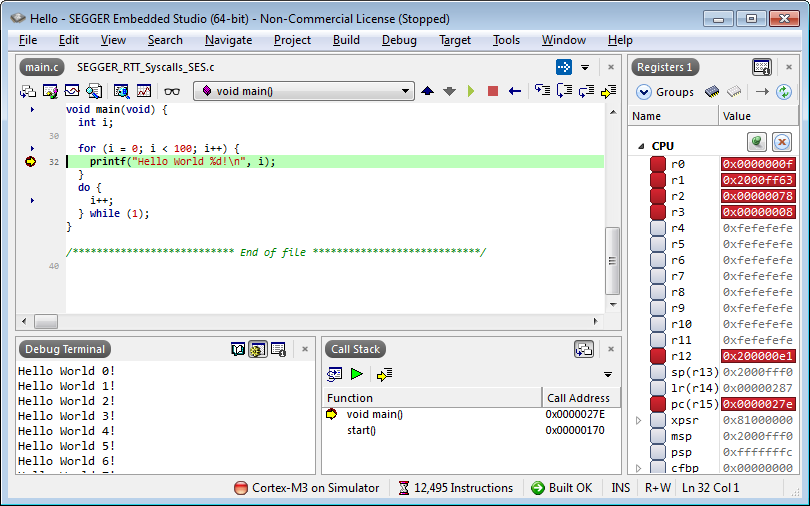
\includegraphics[width=\paperwidth,height=\paperheight]{embedded-studio-debugging.png}
      };
    \end{tikzpicture}
  \end{frame}
}


\begin{frame}[fragile]{Dedykowane IDE dla kontrolera}
  \begin{table}[]
    \begin{tabular}{p{0.5\textwidth}p{0.5\textwidth}}
      \ & \uncover<4->{* to środowisko kontroluje nas,} \\
      \ & \uncover<4->{\ \ a nie my środowisko} \\
      \ & \uncover<3->{* robienie rzeczy, których} \\
      \ & \uncover<3->{\ \ nie przewidzieli twórcy,} \\
      \ & \uncover<3->{\ \ jest trudne (albo niemożliwe)} \\
      \uncover<1->{* klikamy DEBUG} & \uncover<2->{* za każdym razem musimy} \\
      \uncover<1->{\ \ i się debuguje} &  \uncover<2->{\ \ się uczyć od nowa} \\
      \multicolumn{2}{l}{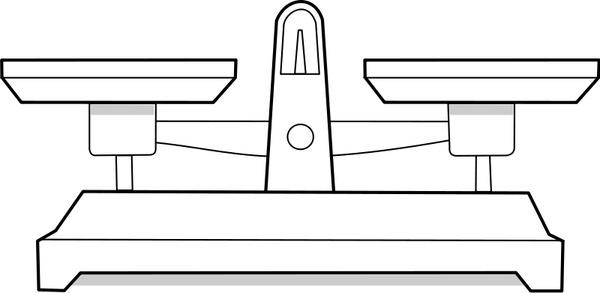
\includegraphics[width=\textwidth, height=4cm]{scales.jpg}}
    \end{tabular}
    \end{table}
\end{frame}

{ % all template changes are local to this group.
  \setbeamertemplate{navigation symbols}{}
  \begin{frame}[plain]
    \begin{tikzpicture}[remember picture,overlay]
      \node[at=(current page.center)] {
        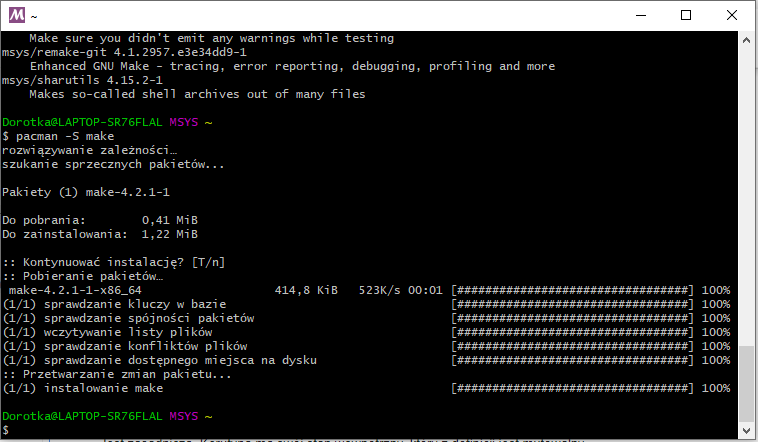
\includegraphics[width=\paperwidth,height=\paperheight]{msys.png}
      };
    \end{tikzpicture}
  \end{frame}
}

\begin{frame}[fragile]{Zagadka - jak nazwać \texttt{f}?}
  \begin{columns}[T] % align columns
    \begin{column}{.38\textwidth}
  
      \begin{Snippet}
(define (f lol)
  (apply map list lol))
      \end{Snippet}
      \pause

      \begin{Snippet}
(list 1 2 3) ===> '(1 2 3)
      \end{Snippet}
      \pause

       \begin{Snippet}
(map + '(1 2 3) '(4 5 6))
   ===> (5 7 9)
      \end{Snippet}
      \pause

      \begin{Snippet}
(apply f '(1 2 3))
 === (f 1 2 3)
      \end{Snippet}
      \pause

      \begin{Snippet}
(apply f 0 '(1 2 3))
 === (f 0 1 2 3)
      \end{Snippet}
      \pause

    \end{column}%
    \hfill%
    \begin{column}{.58\textwidth}
      \begin{Snippet}
def f(lol):
    return map(list, *lol)
      \end{Snippet}
      \pause
      \begin{Snippet}
def list(*elements):
    return elements
      \end{Snippet}
      \pause

      \begin{Snippet}
(apply map list '((1 2 3)
                  (4 5 6)))
      \end{Snippet}
      \pause
      \begin{Snippet}
(map list '(1 2 3) '(4 5 6))
      \end{Snippet}
      \pause
      \begin{Snippet}
'((1 4)
  (2 5)
  (3 6))
      \end{Snippet}

      \pause
      \begin{Snippet}
(f '((1 2 3)
     (4 5 6))) ===> '((1 4)
                      (2 5)
                      (3 6))
      \end{Snippet}
      
    \end{column}%
  \end{columns} 
  
\end{frame}

\begin{frame}[fragile]{Dobre praktyki}
  \begin{itemize}
    \pause
    \item Testy jednostkowe
    \pause
    \item Kod, który działa na kontrolerze, powinno dać się
      również wybudować i uruchomić na PC
  \end{itemize}
\end{frame}

\begin{frame}[fragile]{Struktura projektu embedded}
    \begin{tikzpicture}[remember picture,overlay]
      \node[at=(current page.center)] {
        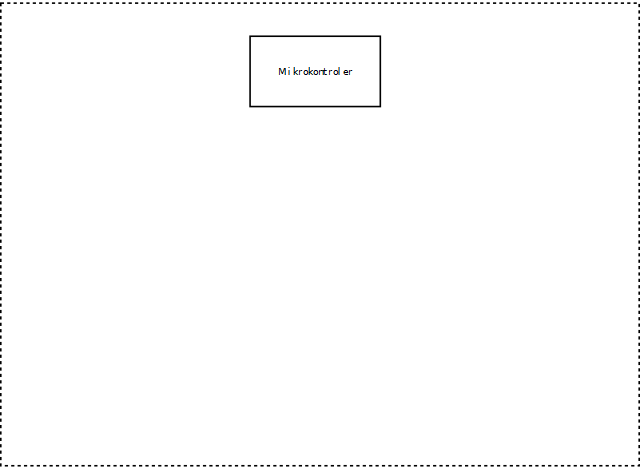
\includegraphics[width=\textwidth]{82.png}
      };
    \end{tikzpicture}
\end{frame}

\begin{frame}[fragile]{Struktura projektu embedded}
    \begin{tikzpicture}[remember picture,overlay]
      \node[at=(current page.center)] {
        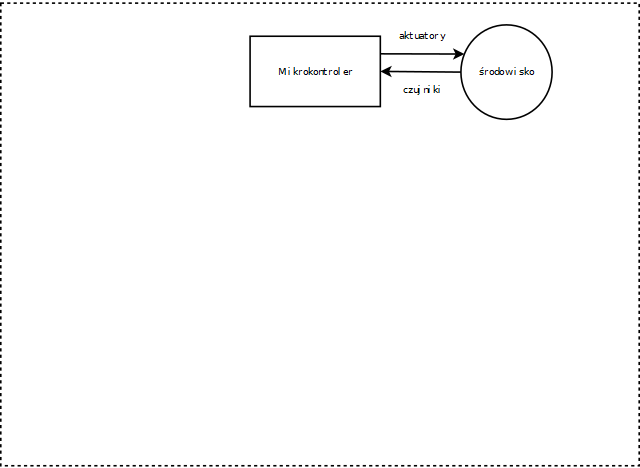
\includegraphics[width=\textwidth]{83.png}
      };
    \end{tikzpicture}
\end{frame}

\begin{frame}[fragile]{Struktura projektu embedded}
    \begin{tikzpicture}[remember picture,overlay]
      \node[at=(current page.center)] {
        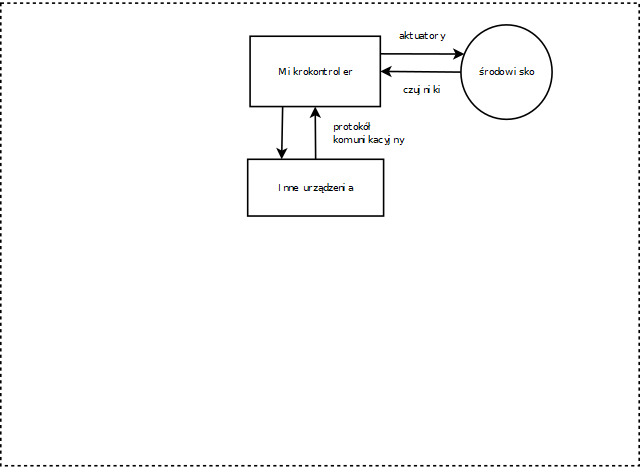
\includegraphics[width=\textwidth]{84.png}
      };
    \end{tikzpicture}
\end{frame}

\begin{frame}[fragile]{Struktura projektu embedded}
    \begin{tikzpicture}[remember picture,overlay]
      \node[at=(current page.center)] {
        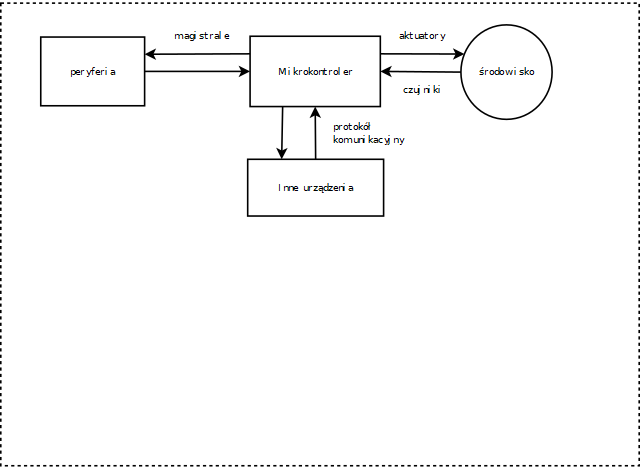
\includegraphics[width=\textwidth]{85.png}
      };
    \end{tikzpicture}
\end{frame}

\begin{frame}[fragile]{Struktura projektu embedded}
    \begin{tikzpicture}[remember picture,overlay]
      \node[at=(current page.center)] {
        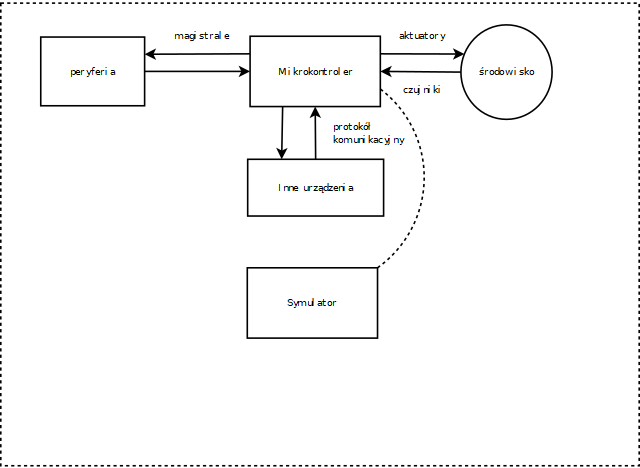
\includegraphics[width=\textwidth]{86.png}
      };
    \end{tikzpicture}
\end{frame}

\begin{frame}[fragile]{Struktura projektu embedded}
    \begin{tikzpicture}[remember picture,overlay]
      \node[at=(current page.center)] {
        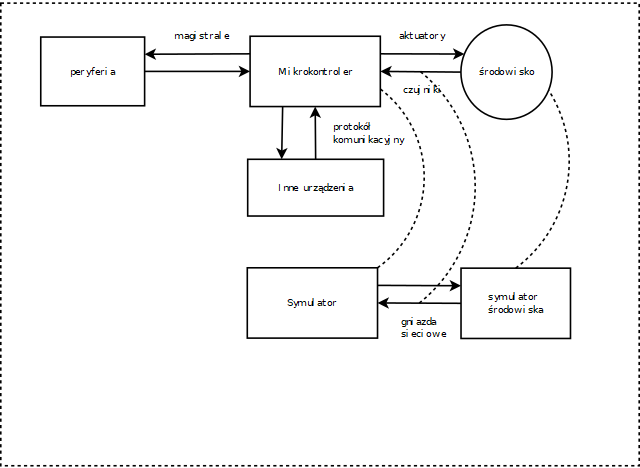
\includegraphics[width=\textwidth]{87.png}
      };
    \end{tikzpicture}
\end{frame}

\begin{frame}[fragile]{Struktura projektu embedded}
    \begin{tikzpicture}[remember picture,overlay]
      \node[at=(current page.center)] {
        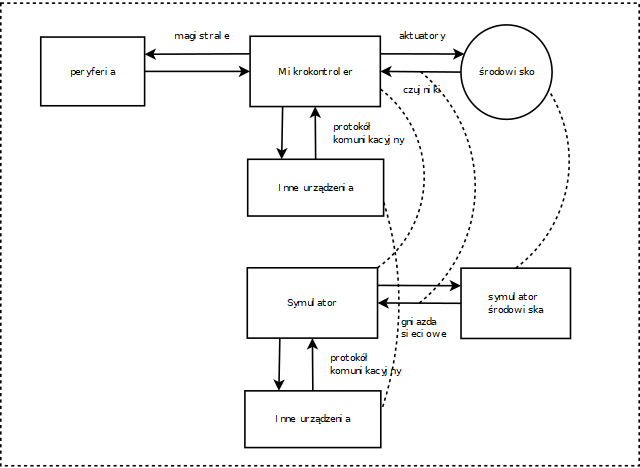
\includegraphics[width=\textwidth]{88.png}
      };
    \end{tikzpicture}
\end{frame}

\begin{frame}[fragile]{Struktura projektu embedded}
    \begin{tikzpicture}[remember picture,overlay]
      \node[at=(current page.center)] {
        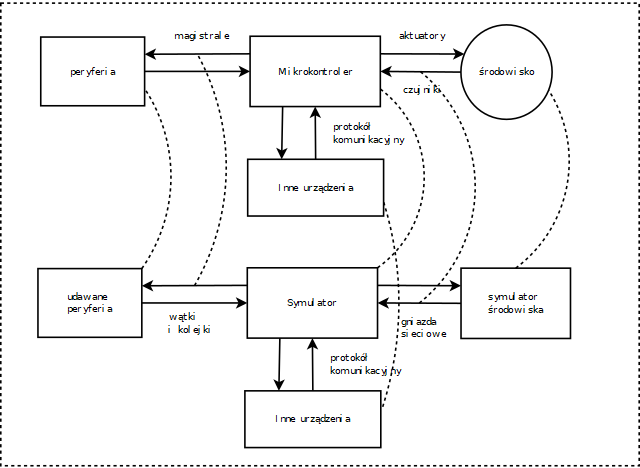
\includegraphics[width=\textwidth]{89.png}
      };
    \end{tikzpicture}
\end{frame}

\begin{frame}[fragile]{Symulator środowiska}
  \begin{Snippet}
    #lang racket
    ;; https://github.com/panicz/praktyki-embedded
  \end{Snippet}
  \pause
  \begin{Snippet}
    (require racket/gui/base racket/tcp
             "grand-syntax.rkt" "ground-scheme.rkt"
             "tcp-server.rkt")
  \end{Snippet}
  \pause
  \begin{Snippet}
    (define simulator-window (new frame%))
  \end{Snippet}
  \pause
  \begin{Snippet}
    (define temperature
      (new slider% [label "Temperatura"]
                   [min-value -273]
                   [max-value 1000]
                   [init-value 20]
                   [style '(vertical vertical-label)]
                   [parent simulator-window]))
  \end{Snippet}
  \pause
  \begin{Snippet}
    (send simulator-window show #true)
  \end{Snippet}
  \pause
  \begin{Snippet}
    (tcp-server 12345
     ("temperature" (send temperature get-value))
     (_ 0))
  \end{Snippet}
\end{frame}

\begin{frame}[fragile]{Korzystanie z gniazd sieciowych}
  \begin{Snippet}
    #include <stdio.h>
    #include <assert.h>
    #include <stdlib.h>
    #include <stdint.h>
    #include <ctype.h>
    #include <string.h>
    #ifdef MINGW
    #  define WIN32_LEAN_AND_MEAN
    #  include <winsock2.h>
    #  include <Ws2tcpip.h>
    #  include <errno.h>
    #else // !MINGW
    #  include <sys/types.h>
    #  include <sys/socket.h>
    #  include <sys/select.h>
    #  include <netinet/in.h>
    #  include <netinet/tcp.h>
    #  include <arpa/inet.h>
    #endif // !MINGW

  \end{Snippet}
\end{frame}

\begin{frame}[fragile]{Korzystanie z gniazd sieciowych}
  \begin{Snippet}
    
int main() {
#ifdef MINGW
  WSADATA wsadata;
  if (WSAStartup(MAKEWORD(1,1), &wsadata) == SOCKET_ERROR) {
    puts("Failed to initialize winsock subsystem");
    return -1;
  }
#endif // MINGW
  \end{Snippet}
  \pause
  \begin{Snippet}
  int sock = socket(AF_INET, SOCK_STREAM, IPPROTO_TCP);
  assert(sock >= 0);

  struct sockaddr_in address;
  address.sin_addr.s_addr = inet_addr("127.0.0.1");
  address.sin_family = AF_INET;
  address.sin_port = htons(12345);

  int error = connect(sock, (struct sockaddr *) &address,
                      sizeof(address));
  assert(!error);
  \end{Snippet}
\end{frame}
  
\begin{frame}[fragile]{Korzystanie z gniazd sieciowych}
  \begin{Snippet}
      char line[255];
      char response[255];
      while (1) {
        fgets(line, sizeof(line), stdin);
        int sent = send(sock, line, strlen(line), 0);
        int received = recv(sock, response,
                            sizeof(response), 0);
        response[received] = '\0';
        printf("%s", response);
        fflush(stdout);
      }
      return 0;
    }
  \end{Snippet}
\end{frame}

\begin{frame}[fragile]{\texttt{Makefile}}
  \begin{Snippet}
    HOST_OS = $(shell uname -o)

    ifeq ($(HOST_OS), Msys)
      LIBS = -mwindows -lws2_32 -lmingw32 -DMINGW
    endif

    all: tcpclient

    tcpclient: cl.c
        gcc $(CFLAGS) $< -o $@ $(LIBS)

    clean:
        rm tcpclient
  \end{Snippet}
\end{frame}
    

\begin{frame}[fragile]{W docelowym kodzie}
  \begin{Snippet}
#include "config.h" // definiuje stale DEVICE i SIMULATOR
    
int current_temperature_C(void) {
  int temperature_C = 20;
  \end{Snippet}
  \pause
  \begin{Snippet}
#if TARGET == SIMULATOR
  int n = send(sock, "temperature",
               sizeof("temperature"), 0);
  assert(n == sizeof("temperature"));
  char buffer[16];
  n = recv(sock, buffer, sizeof(buffer), 0);
  assert(n > 0 && n < 16);
  buffer[n] = '\0';
  sscanf(buffer, "%d", &temperature_C);
  \end{Snippet}
  \pause
  \begin{Snippet}
#elif TARGET == DEVICE
  i2c_read(temperatureSensor, &temperature_C);
  \end{Snippet}
  \pause
  \begin{Snippet}
#else
#  error "Unknown target"
#endif // TARGET
  return temperature_C;
}
  \end{Snippet}
\end{frame}


\begin{frame}[fragile]{Sterownik wyświetlacza - struktura}
  \begin{Snippet}
struct {
  // ...
#if TARGET==SIMULATOR      
  SDL_Window *window;
  SDL_Surface *surface;
  pthread_t sync_screen;
  uint32_t LTDC_CLUT[256];
#endif // TARGET==SIMULATOR
  // ...
  uint8_t videobuffer[SCREEN_HEIGHT][SCREEN_WIDTH];
  // ...
} Global;
  \end{Snippet}
\end{frame}

\begin{frame}[fragile]{Sterownik wyświetlacza - inicjalizacja}
  \begin{Snippet}
int main(void) {
// ...      
#if TARGET == SIMULATOR
  SDL_Init(SDL_INIT_VIDEO);
  Global.window =
    SDL_CreateWindow("embedded device",
                     SDL_WINDOWPOS_UNDEFINED,
                     SDL_WINDOWPOS_UNDEFINED,
                     SCREEN_WIDTH, SCREEN_HEIGHT,
                     0);
  Global.surface = SDL_GetWindowSurface(Global.window);
  assert(Global.surface);
  pthread_create(&Global.sync_screen, NULL,
                 LTDC_SDL_sync, NULL);
#endif // TARGET == SIMULATOR  
  // ...
}
  \end{Snippet}
\end{frame}


\begin{frame}[fragile]{Sterownik wyświetlacza - symulacja}
  \begin{Snippet}
void *LTDC_SDL_sync(void *unused) {
  while (1) {
    uint32_t *pixels = (uint32_t *) Global.surface->pixels;
    for (int line = 0; line < SCREEN_HEIGHT; ++line) {
      for (int pixel = 0; i < SCREEN_WIDTH; ++pixel) {
            pixels[line*SCREEN_WIDTH + pixel] = 
              Global.LTDC_CLUT[
                Global.videobuffer[line*SCREEN_WIDTH + pixel]
              ];
          }
        }
        SDL_UpdateWindowSurface(window);
      }
      if (line == sync_line) {
        LTDC_LineEvent();
      }
    }
  }
  return NULL;
}
  \end{Snippet}
\end{frame}




    
\end{document}
